\chapter[Metodologia]{Metodologia}\label{cap3}

\section{Levantamento Bibliográfico}

A pesquisa bibliográfica foi feita, basicamente, por assunto, por autor e por título. A pesquisa realizada por assunto foi a mais utilizada e termos adequados foram usados para se obter um pesquisa mais efetiva para o entendimento e desenvolvimento do trabalho tais como \textit{audiobooks}, não-videntes, deficientes visuais, educação, ogg vorbis, livorbisfile, libvorbis, libvorbisenc, compressão de áudio, formatos de áudio, WAV, AIFF, MP3, PCM, entre outros. Também foram feitas pesquisas por assunto a respeito de ferramentas necessárias para o desenvolvimento do trabalho tais como fórmulas latext, player ogg, sox play, dump ogg, bibtex models example, Qt Creator e Qt Designer, entre outros. Para a pesquisa feita por autor e título é necessário que já se saiba qual autor ou obra são relevantes para o tema escolhido como, por exemplo, a pesquisa pelo autor Tanenbaum. Levantamento por assunto foi bastante utilizado em pesquisa na internet usando catálogos e mecanismos de busca em sites como o Google Acadêmico \cite{googleacademico}, Google com pesquisa \textit{web} e com filtro para livros, \textit{ACM Digital Library} \cite{acm} e Scielo \cite{scielo}. Ideias e dicas dadas pelo prof. Dr. Edson Júnior foram de suma importância principalmente para uma determinação de ``um ponto de partida''.

Através do levantamento bibliográfica foi possível listar e consolidar citações de trabalhos fundamentais para o tema ou algo similar ao que foi proposto neste trabalho.

\section{Ferramentas utilizadas}

As ferramentas utilizadas para o desenvolvimento do trabalho são descritas, em poucas palavras, para qual propósito cada uma foi usada e qual a versão utilizada.

Por fornecer ferramentas nativas que ofereceram grande suporte para o desenvolvimento deste trabalho, pelo formato Ogg Vorbis fornecer API de fácil instalação e uso em distribuições Unix e pelo conhecimento prévio dos sistemas operacionais o Ubuntu 14.04 LTS foi adotado para um primeiro momento e o OS X Yosemite versão 10.10.4 para um segundo momento para o ambiente de desenvolvimento. O uso dos dois sistemas não influenciou no desenvolvimento, ambos são distribuição Unix sendo pessoal o fator motivacional. O compilador utilizado foi o gcc versão 4.8.2.

O editor de texto utilizado para o desenvolvimento dos códigos fonte em linguagem de programação C foi o Sublime Text 2. Ele foi escolhido por possuir uma interface limpa, por fornecer uma prévia visualização de todo o documento e, principalmente, pelos comandos que ele oferece para facilitar a codificação. Podemos citar como exemplo a troca de linhas sendo possível mover uma linha ou um bloco inteiro de código, cursores múltiplos possibilitando a escrita em diversas parte do código simultaneamente, busca por palavras de mesmo nome e a busca e substituição de palavras específicas com uma ou múltiplas seleções.

O Latex foi utilizado para desenvolver o trabalho escrito e escolhido por gerar, como saída, um pdf com alta qualidade tipográfica e totalmente formatado. A versão utilizada foi pdfTeX versão 3.1415926-2.5-1.40.14.

Inicialmente foi utilizada a ferramenta hexdump nativa do sistema operacional Unix para mostrar os dados binários em hexadecimal com o intenção de facilitar o entedimento do formato de áudio e validar os dados inseridos posteriormente. Entretanto, a feramenta hexdump foi substituída pela oggz versão 1.1.1 por aprensentar de forma mais limpa e segmentada os pacotes do formato Ogg e por conter informações adicionais como: número do pacote, tamanho do pacote, sequência, dentre outras.

A versão v.14.4.1 da ferramenta sox foi utilizada para executar os arquivos de áudio *.ogg com o intuito de verificar se o arquivo não foi corrompido devido as constantes modificações do formato para inserção do pacote de marcação de conteúdo e da inserção dos metadados no cabeçalho de comentários.

A biblioteca libvorvis foi utilizada como suporte ao uso da compressão de dados e integrada no Editor desenvolvido. A rotina é capzar de comprimir os dados contidos no formato e sua posterior recuperação.

O Qt Designer 5.4.2 foi utilizado para a construção da interface gráfica da aplicação que executa o formato especificado. O Tocador foi desenvolvido em C++ e, para execução do áudio, a rotina do framework SDL (Simple Directmedia Layer) versão 1.2.15 foi configurada e integrada na aplicação. O QtSpeech foi utilizado como suporte ao uso de sintetizador de voz no Tocador e é capaz de utilizar a voz sintetizada do próprio sistema operacional.

O Qt é um framework multiplataforma que possui deversos módulos para desenvolvimento de software. Como alguns módulos do Qt foram utilizados para a construção do Tocador e de sua interface gráfica, tais como QtCore, QtGui, QtWidgets e QtDesigner, para a cobertura de testes, o módulo QtTest foi selecionado para a implementação dos testes unitários.

Para o controle de versão, o GitHub foi a ferramenta utilizada. O projeto está acessível em \href{https://github.com/BryanFernandes/player_rab-ogg}{BryanFernandes/player\_rab-ogg}.

Dada a complexidade para a montagem do ambiente de desenvolvimento viu-se a necessidade de automatiza-lo. Dessa forma, o próprio sistema operacional será o responsável por construir um ambiente capaz de compilar, executar e testar o Tocador. Com suporte aos sistemas operacionais OS X e Linux, o Vagrant foi a ferramenta escolhida para este fim. A partir de um script, ele é capaz de criar e recriar ambientes em qualquer lugar de forma simples e descomplicada. Para isso, o Vagrant faz uso das soluções de virtualização mais comuns como o Virtualbox que será utilizado neste trabalho.

A ferramenta CodeClimate foi utilizada para garantir uma melhor qualidade de código e prevenção de potenciais \textit{bugs}. Esta ferramenta realiza a análise estática do código fonte e notifica a equide de desenvolvimento quando potenciais bugs podem ocorrer no projeto. A ferramenta também é capaz de manter um registro das \textit{issues} encontradas.

Por apresentar fácil utilização e integração com outros sistemas, o Travis CI foi a ferramenta escolhida para automação do processo e engenharia do produto. A ferramenta integra-se ao GitHub indicando quando em cada commit ocorreu sucesso ou falha no processo de automatção. o Travis também mantém um histórico com logs das execuções realizadas além de notificar por e-mail a equipe de desenvolvimento ao final de cada execução realizada.

\section{Proposta anterior}

A proposta de solução foi baseada no trabalho desempenhado por \cite{herbert}. Como ponto inicial ao desenvolvimento da solução tecnológica, a primeira coisa a ser feita foi entender a proposta de \cite{herbert} e, para isso, foi feito um estudo em cima de sua monografia. Conforme documentado, o sistema possuem três componentes, sendo eles: o Tocador, o Editor RAB e o Core como mostra a Figura \ref{components}.

 \begin{figure}[ht]
	\centering
		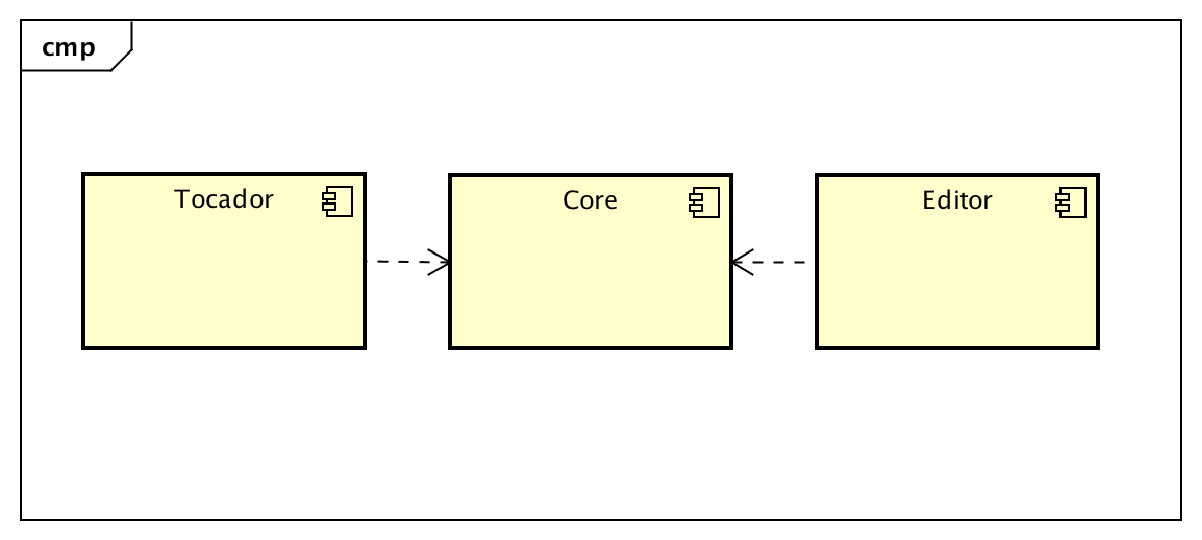
\includegraphics[keepaspectratio=true,scale=0.5]{figuras/components.eps}
	\caption{Diagrama de Componentes.}
	\label{components}
\end{figure}

O Core é a biliboteca estática comum e importante ao funcionamento do Tocador e do Editor. A Figura \ref{core} apresenta a biblioteca estática de forma mais detalhada. 

 \begin{figure}[ht]
	\centering
		\includegraphics[keepaspectratio=true,scale=0.5]{figuras/core.eps}
	\caption{Diagrama de Classe do Core.}
	\label{core}
\end{figure}

O diagrama de classes do Tocador está representado na Figura \ref{tocador}. O componente foi separado nas camadas Modelo, Visão e Controladora segundo o padrão MVC. O pacote core representa a biblioteca estática.

\begin{figure}[ht]
	\centering
		\includegraphics[keepaspectratio=true,scale=0.4]{figuras/tocador.eps}
	\caption{Diagrama de Classe do Tocador.}
	\label{tocador}
\end{figure}

E, por fim, a Figura \ref{editor} mostra o diagrama de classe do Editor. A classe \textit{Main} utiliza os serviços das classes da biblioteca Core e implementa as funções de iteração com usuário através de linha de comando.

\begin{figure}[ht]
	\centering
		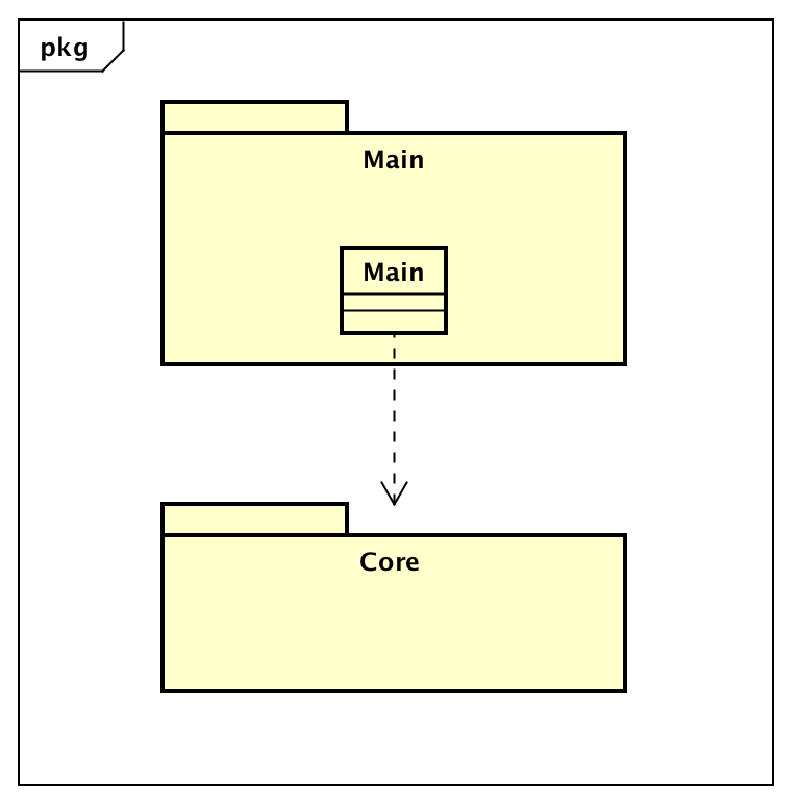
\includegraphics[keepaspectratio=true,scale=0.5]{figuras/editor.eps}
	\caption{Diagrama de Classe do Editor RAB.}
	\label{editor}
\end{figure}

A proposta de melhoria para o trabalho anterior considerou os problemas levantados e traçou, como objetivo, uma proposta inovadora sobre os aspectos sociais, econômicos, tecnológico e, principalmente, sobre a inclusão de pessoas que possuam alguma limitação para uso do sistema. Portanto, a solução trata da inclusão social dos deficientes visuais oferecendo a eles suporte ao ensino com baixo custo do uso da tecnologia.

%apenas o software em si, mas também todo o processo de desenvolvimento. Foi levado em consideração os pontos fortes e fracos levantados pelo autor. O autor propôs, inicialmente, o uso de alguns artefatos do RUP e algumas práticas da metodologia ágil. No entanto, como o prazo era curto e a equipe de desenvolvimento era composta por apenas uma pessoa, o processo, de um modo geral, foi ad hoc. Isto explica o fato de ele não ter seguido o que o processo RUP especifica, a saber, a separação das atividades desenvolvidas em Concepção, Elaboração, Construção e Transição. Assim sendo, o processo utilizado também foi ad hoc.

\section{Entendendo o Ogg Vorbis}

O segundo passo foi o estudo de um novo formato: Ogg Vorbis desenvolvido pela fundação Xiph.org. Foi feito um estudo minucioso em cima do documento de especificação do formato Ogg Vorbis para conhecer a sua estrutura e o tipo de suporte que ele oferece. A ferramenta \textit{hexdump} utilizada por \cite{herbert} foi usada como suporte para um melhor entendimento do formato *.ogg. A Figura \ref{hexdump} mostra o resultado da execução do hexdump em um arquivo *.ogg cujo comando é: \$ hexdump -C <file\_name>.

 \begin{figure}[ht]
	\centering
		\includegraphics[keepaspectratio=true,scale=0.5]{figuras/hexdump.eps}
	\caption{Execução da ferramenta hexdump.}
	\label{hexdump}
\end{figure}

No entanto, os dados ainda ficaram muito confusos e de difícil interpretação. Após uma pesquisa verificou-se a existência de uma outra ferramenta também nativa no sistema operacional Ubuntu e voltada para os arquivos com extensão *.ogg e possui a mesma finalidade da ferramenta hexdump. A diferença entre elas está na forma com que os dados são apresentados. Podemos verificar na Figura \ref{oggzdump} como o oggz-dump estrutura os dados. O comando para execução da ferramenta é dado no terminal e possui o seguinte formato: \$ oggz-dump <file\_name>.

 \begin{figure}[ht]
	\centering
		\includegraphics[keepaspectratio=true,scale=0.5]{figuras/oggz-dump.eps}
	\caption{Execução da ferramenta oggz-dump.}
	\label{oggzdump}
\end{figure}

É notável a diferença e a facilidade com que a ferramenta oggz informa sobre os pacotes contidos em um arquivo *.ogg. Após o comando é possível verificar os pacotes separadamente bem como sua informações tais como número do pacote, informações de grânulo, o ``tempo'' em que aquele pacote é lido, o seu tamanho, entre outras informações. Além das informações do pacote também é possível visualizar seu conteúdo e logo percebemos que os pacotes de número 0, 1 e 2 são os pacotes cabeçalhos. A identificação dos pacotes cabeçalhos pode ser percebida pois após o primeiro byte do pacote, os 6 bytes subsequentes contém a string ``vorbis'' onde cada byte representa uma letra.

\section{Desenvolvimento do Editor}

\subsection{Construção do codificador}

O estudo e o processo acima foi realizado para entender a estrutura do Ogg Vorbis e onde inserir os metadados e as marcações de conteúdo validando, assim, a possibilidade do uso do formato para a solução do problema. Para dar continuidade no estudo de viabilidade do formato Ogg Vorbis, foi desenvolvido um codificador em linguagem C. Como suporte, foram utilizadas as bibliotecas \textit{libogg}, \textit{libvorbis} e \textit{libvorbisenc}. O \textit{libvorbisenc} é responsável pela codificação. Para compilar o arquivo é necessário utilizar o seguinte comando: 
	
   
   \$ gcc -o <nome\_para\_o\_executável> <código\_fonte> -logg -lvorbis -lvorbisenc


Para garantir que o processo de codificação realmente funcionasse, foi utilizado outro formato no processão de codificação de um formato Ogg Vorbis. O código desenvolvido pega o conteúdo sonoro de um formato WAVE e o codifica em Ogg Vorbis, com os seus dados comprimidos. Em outras palavras, o PCM do formato WAVE é decodificado e posto em memória e, em seguida, os pacotes cabeçalhos do Ogg Vorbis são construídos. O PCM passa a ser inserido dentro do pacote de áudio finalizando o processo de decodificação. A ferramenta \textit{oggz-dump} foi executada no arquivo gerado e após análise, os pacotes cabeçalhos, em tese, foram codificados corretamente. Para verificar se a integridade do arquivo não foi corrompida, utilizou-se o player Sound Exchange licenciado sob a GNU General Public License e distribuído por Chris Bagwell através \cite{sox}. Este player possui uma interface de linha de comando e, ao utilizá-lo, era possível executar o som, este agora no formato Ogg, sem interrupção. 

%O arquivo WAVE ocupava um espaço de 1.4MB em memória e após a codificação, o arquivo Ogg Vorbis ocupou apenas 86kb.


%A decisão para uso deste formato foi de rápida aceitação pois, além de ser open source, ele possui licença BSD e seu formato faz uso de compressão de dados.

\subsubsection{Inserção dos metadados}

Como fundamentado teoricamente no item mais acima, o arquivo *.ogg possui um pacote onde é possível inserir comentários. O \textit{comment packet} é o segundo pacote de cabeçalho da sequência de três que o Ogg Vorbis utiliza. Na Figura \ref{oggzdump} ele aparece como o pacote número 1. O próximo passo então foi inserir, comentários referentes ao arquivo de áudio. Logo, o pacote de comentários do formato Ogg Vorbis foi utilizado para inserção dos metadados e, comparando-o ao trabalho realizado \cite{herbert}, corresponde a estrutura META. Para este fim, o código desenvolvido em linguagem de programação C para a codificação foi modificado e este agora, além de pegar o conteúdo sonoro de um formato WAVE e o codificar em Ogg Vorbis com os dados comprimidos, ele também insere metadados no pacote. Para verificação da integridade do arquivo neste ponto do desenvolvimento, os mesmos passos utilizados no processo de codificação foram seguidos e as ferramentas \textit{oggz-dump} e \textit{sox} foram utilizadas.

\subsubsection{Construção do pacote LGMK}

Referente a estrutura LGMK \cite{herbert}, o formato Ogg Vorbis não possui suporte e se fez necessário a alteração de sua estrutura. Isso deveria ser feito, obviamente, sem que o arquivo fosse corrompido possibilitando sua execução em players comuns. Para tal finalidade, um novo pacote foi definido. A Figura \ref{lgmk} mostra quais são os campos que compõe o pacote.

 \begin{figure}[ht]
	\centering
		\includegraphics[keepaspectratio=true,scale=0.8]{figuras/lgmks.eps}
	\caption{Formato do pacote LGMK.}
	\label{lgmk}
\end{figure}

O campo referente ao \textbf{user\_lgmks} é um array que armazena todas as marcações fornecidas pelo usuário e seu tamanho é ilimitado. O \textbf{lgmks\_lengths} é um array responsável por armazenar o tamanho de cada marcação. A quantidade de marcações contidas no campo user\_lgmks é armazenada no \textbf{lgmks}. Por último, o campo \textbf{user} contém informações sobre o usuário que fez as marcações. Uma nova estrutura foi definida e inserida dentro do formato sem, obviamente, corrompê-lo. Foi possível codificar e também decodificar as marcações de conteúdo com integridade.

Os três \textit{header packets} definidos pelo Vorbis devem seguir a ordem disposta na Figura \ref{newformat} ou o arquivo será corrompido. O pacote LGMK não é reconhecido pelo Vorbis pelos seguintes motivos:

\begin{enumerate}
	\item O pacote possui um tipo diferente dos três tipos de cabeçalhos do Vorbis, desta forma ocorre erro no processo de decodificação.
	\item A string de identificação do pacote é ``lgmks'' e o Vorbis não irá decodificar este pacote;
	\item Quando o Vorbis for decodificar o pacote de áudio, o pacote LGMK SERÁ ignorado por ser um pacote não-áudio.
\end{enumerate}

 No entanto, a decodificação não é corrompida por conta da forma que foi estruturado o pacote e do local onde foi inserido. O pacote LGMK foi construído como sendo um pacote de cabeçalho semelhante aos \textit{header packets} do \textit{codec} Vorbis. Ou seja, ele possui um byte para a identificação do tipo de pacote de cabeçalho. A diferença está nos seis bytes subsequentes, onde a string que representa a identificação do pacote é ``lgmks''. O pacote foi inserido direto no formato recipiente Ogg logo após o terceiro pacote de cabeçalho do Voribs. A Figura \ref{newformat} mostra como ficou organizado a estruturação do formato Ogg vorbis após inserção do pacote referente a marcação de conteúdo.

\begin{figure}[ht]
	\centering
		\includegraphics[keepaspectratio=true,scale=0.8]{figuras/newformat.eps}
	\caption{Estrutura Ogg Vorbis com o pacote LGMK inserido.}
	\label{newformat}
\end{figure}

Como foi posto após o cabeçalho de configuração do Ogg Vorbis, no processo de decodificação padrão, o pacote LGMK tentará ser codificado como pacote de áudio e então será ignorado. Portanto, ao executar um player o arquivo Ogg Vorbis gerado é tocado normalmente.

\subsection{Construção do decodificador}

Para o desenvolvimento do código referente ao processo de decodificação do arquivo *.ogg foram utilizadas as bibliotecas \textit{libvorbisfile}, \textit{libvorbis} e \textit{libogg}. A \textit{libvorbisfile} oferece o suporte necessário voltado para a decodificação do arquivo tornando o processo mais simples. Para compilar o arquivo é necessário utilizar o seguinte comando: 
	
   \$ gcc -o <nome\_para\_o\_executável> <código\_fonte> -logg -lvorbis -lvorbisfile

O código implementado decodifica os dados de cabeçalho e os imprime no terminal. Os dados PCM contidos do pacote de áudio são direcionados para um arquivo de saída.

\subsubsection{Decodificação dos metadados}

O metadados, uma vez codificados, precisavam ser decodificados e seu conteúdo recuperado em mémoria sem perda de dados. Para este fim, foi feito o uso da API \textit{libvorbisfile} onde foi possível recuperar os metadados corretamente.

\subsubsection{Decodificação do pacote LGMK}

Como dito, o pacote é inserido diretamente no contêiner Ogg, ou seja, em nenhum momento é feito uso da estrutura vorbis para a inserção do pacote. Para o processo de decodificação do pacote LGMK, e por não fazer parte da estrutura Vorbis, a biblioteca \textit{libvorbisfile} não oferece nenhum suporte e foi desconsiderada no processo de decodificação a partir deste ponto do projeto. Para alcançar o objetivo de decodificação, o uso das bibliotecas \textit{libvorbis} e \textit{logg} foram ainda mais efetivos. A \textit{libvorbis} ainda foi utilizada para decodificar a estrutura Vorbis, porém de uma forma mais ``manual''. Para o pacote LGMK foi utilizada apenas a biblioteca \textit{logg}. Ao final, todo o arquivo foi decodificado corretamente.

\subsection{Diagrama de Classe do Editor}

Seguindo a arquitetura anterior, a Figura \ref{editorogg} apresenta o diagrama de classe para o Editor OGG desenvolvido conforme especificado nas sessões anteriores.

\begin{figure}[ht]
	\centering
		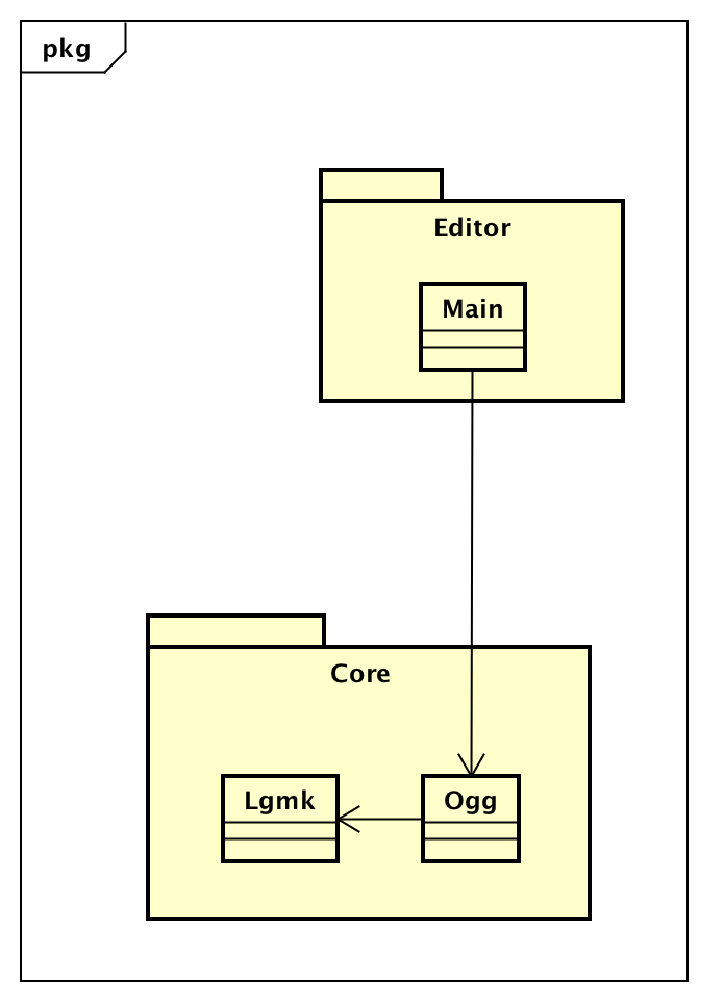
\includegraphics[keepaspectratio=true,scale=0.5]{figuras/editorogg.eps}
	\caption{Diagrama de classe do Editor OGG.}
	\label{editorogg}
\end{figure}

Recorrendo aos serviços oferecidos pelo Core, a classe \textit{Main} é responsável por abrir um arquivo OGG, construir o pacote de marcação e gerar, como saída, o formato com o pacote em sua estrutura. A classe \textit{Ogg} é responsável por codificar e decodificar o formato. A construção do pacote de marcação está contido dentro da classe \textit{Lgmk}. Tanto o pacote \textit{Lgmk} quanto o pacote \textit{Ogg} foram postos no Core do sistema pois estes serão necessários também para a execução do formato no Tocador.

\section{Desenvolvimento do Tocador}

O tocador foi inicialmente desenvolvido por \cite{herbert} oferecendo suporte apenas aos formatos WAV e RAB. Desenvolvido em C++, o tocador faz uso do Qt para interfaceamento da apliacação e foi modificado originalmente para oferecer suporte ao novo formato comprimido especificado. A manutenção e evolução feita no Player está disseminada em boa parte do código visto que o Player passou a ser alimentado por este novo formato. O Tocador passou a fazer o uso da rotina libvorbis para descompressão dos dados e da API desenvolvida neste trabalho representada pelo Editor para a decodificação dos metadados e suas marcações. Referente a execução do áudio, para que fosse executado corretamente e os saltos fossem precisos, o cálculo para interpretação dos bytes do PCM do áudio decodificado foi reformulado. Na Figura \ref{layout} está representado a interface do Tocador proposta por \cite{herbert}:

\begin{figure}[ht]
	\centering
		\includegraphics[keepaspectratio=true,scale=0.4]{figuras/layout.eps}
	\caption{Layout do Tocador estruturado pela ferramenta Qt Desginer.}
	\label{layout}
\end{figure}

O Tocador é responsável por informar todos os dados contidos no formato. Os rótulos estáticos \textit{Title, Author, Language, Publisher, Address, Pages e Year} indicam as informações referentes aos metadados do pacote \textit{META} que, por sua vez, estão representados pelos \textit{labels} \textit{\textbf{TitleLabel, AuthorLabel, LanguageLabel, PublisherLabel, AddressLabel, PagesLabel e YearLabel}}. O rótulo \textit{Level} representa os dois possíveis níveis da marcação no que pode ser comparado aos capítulos e subcapítulos de um livro impresso tornando o acesso a informação mais preciso e coerente. \textit{Mark} e \textit{SubMark} são os rótulos responsáveis por informar a marcação e submarcação atual em que o áudio está contido. Ao final do layout tem-se uma barra para navegação manual do áudio e um visor digital que é atualizado constantemente mantendo a informação de tempo em segundos em que a execução do áudio se encontra.

Para fins de acessibilidade para pessoas que possuam limitação visual, o Tocador passou por melhorias de inteface e novas funcionalidades foram inseridas na aplicação. A elicitação dos novos requisitos, a análise destes requisitos e suas escolhas estão dispostos a seguir.

\subsection{Elicitação de Requisitos de Acessibilidade}

%Para este fim, foi realizado um levantamento de softwares existentes que são acessíveis para cegos e pessoas com baixa visão.

Para uma melhor precisão na escolha das funcionalidades que melhor contribuem para utilização de sistemas por pessoas com deficiência visual, 13 sistemas que contemplam este domínio foram analisados: \textit{Blind’s Music Player}, \textit{Dolphin SuperNova Access Suite}, \textit{JAWS}, \textit{LianeTTS}, \textit{MAGic}, \textit{MECDAISY}, \textit{NVDA Screen Reader}, \textit{Projeto DOSVOX}, \textit{Virtual Vision} e \textit{Windows-Eyes}. Segundo o processo proposto por (sommerville), os requisitos foram coletados, classificados e organizados em grupos coerentes. As funcionalidades comuns aos sistemas foram contados e priorizados considerando a funcionalidade de maior frequência como mais importantes:

\begin{figure}[ht]
	\centering
		\includegraphics[keepaspectratio=true,scale=0.3]{figuras/features.eps}
	\caption{Mapeamento das funcionalidades em comum.}
	\label{features}
\end{figure}

A funcionalidade de suporte ao braille, apesar da frequência, não foi implementada por estar fora do escopo e propósito do trabalho aqui desenvolvido. As 7 funcionalidades de maior frequência foram implementadas, das quais são: sintetizador para leitura de tela, contraste de tela, sintetizador para informação de conteúdo, sintetizador para ajuda, destaque visual, ampliador de tela e anúncio automático de texto sob o mouse. Por intermédio destas \textit{features} o cego ou a pessoa com baixa visão consegue acessar todas as informações referente ao \textit{audiobook} que está sendo executado além de oferecer suporte de ajuda para utilização do Tocador.

\subsection{User Stories}

As \textit{features} elicitadas estão representadas em \textit{User Stories} e disponíveis no \hyperref[userstories]{Apêndice A}. Os Critérios de Aceitação para cada \textit{User Story} estão disponíveis no \hyperref[criterios]{Apêndice B}.

\subsection{Codificação}

Após a elicitação, análise e definição dos requisitos o passo seguinte foi a implementação destes no sistema. Os três recursos básicos necessários para inserção das \textit{features} de acessibilidade estão descritos nas sessões seguintes. A descrição de cada funcionalidade e o recurso e suporte que elas dispõem estão detalhados na seção \hyperref[cap4]{Resultados Alcançados}.

\subsubsection{Sintetizador de Voz}

Após a elicitação dos requisitos percebeu-se a necessidade do uso de recurso de voz para a aplicação. Para garantir que o recurso de voz funcionasse e estivesse bem integrado a aplicação foi utilizado a API QtSpeech, pois a ferramenta Qt já faz suporte ao desenvolvimento do Tocador. No entanto, foi utilizado uma versão modificada por Taodyne da biblioteca QtSpeech. Para uso do \textit{tao-qt-speech} o \href{https://github.com/c3d/tao-qt-speech.git}{código fonte} acessível disponibilizado no github foi baixado e os comandos \textit{make} e \textit{make install} foram executados, nesta ordem, para instalação. Ela foi selecionada por fazer integração do suporte QtSpeech ao sintetizador de voz do próprio sistema em que a aplicação está sendo executada, sejam eles Mac OS X, Linux ou Windows.


\subsubsection{Detectando Elementos de Interface}\label{detect}

Para a correta implementação dos requisitos elicitados fez-se necessário a detectação e a diferenciação dos elementos dispostos na interface. Dependendo do elemento que estiver sob o mouse, o texto será ampliado ou os botões disponíveis serão falados e destacados visualmente. Para tal recurso o \textit{EventFilter} é capaz de filtrar os objetos que estão sob o mouse fazendo diferenciação entre eles. O \textit{EventFilter} deve ser instalado em cada objeto através do método \textit{QObject::installEventFilter()}. Após isso, o método \textit{eventFilter(QObject *object, QEvent *event)} fica responsável por escutar os objetos. Esta funcionalidade foi implementada na classe Ui\_meta na camada \textit{View} do Tocador como mostrado na Figura \ref{diagram}.

\subsubsection{Recurso de Teclado}

A definição das teclas funcionais para o Tocador também foram elicitadas a partir do reuso de requisitos na qual os requisitos de layout do teclado dos softwares citados foram analisados. Observou-se que não existe teclas específicas para cada funcionalidade de acessibilidade a pessoas com deficiência visual. No entanto, constatou-se que a tecla definida para dada funcionalidade é representada pela primeira letra do nome daquela funcionalidade, quando disponível. A fim de detectar quando uma tecla é pressionada e atribuir-lhe uma ação, os serviços das classes \textit{QKeyEvent} e \textit{QShortcut} do Qt foram utilizados por oferecerem o suporte necessário. A primeira coisa feita foi obter um referência de uma tecla por intermédio da classe \textit{QKeySequence} que é responsável por encapsular uma tecla ou uma sequência delas para serem usadas com atalho no Tocador. Em seguida, a classe \textit{QShortcut} cria um atalho que associa a tecla ao Tocador. Este atalho, por sua vez, foi conectado a um dado método que será executado no momento em que a tecla for pressionada. Estes passos foram implementados na controladora Player de acordo com a Figura \ref{diagram}.

O método \textit{setControl(SoundCTRL *control)} habilita as teclas e as associa aos métodos da classe \textit{SoundCTRL} da qual é responsável pelo controle do Tocador.

\subsection{Diagrama de Classe do Tocador}

Para a inserção dos requisitos de acessibilidade, dois métodos foram criados na controladora do Tocador. O primeiro deles é o \textit{setKeyboardControl()}. Este método é responsável por criar os atalhos de teclado que executará os métodos de controle de execução do Tocador da classe SoundCTRL. O segundo método é o \textit{setAccessibilitySupport()} cuja função é criar atalhos de teclado para os recursos visuais e do sintetizador de voz que estão definidos na classe Accessiblity. A diagrama de classe está representado na Figura \ref{diagram}.

\begin{figure}[ht]
	\centering
		\includegraphics[keepaspectratio=true,scale=0.3]{figuras/diagram.eps}
	\caption{Diagrama de Classe do Tocador com os recursos de acessibilidade.}
	\label{diagram}
\end{figure}

Para detecção do movimento do mouse e distinção entre os elementos sob ele os métodos \textit{eventFilter()} e \textit{setEventFilter()} foram implementados na classe Ui\_Meta conforme dito na seção \ref{detect}

%\subsection{Engenharia de Produto}

%Para tornar o ambiente automatizado e a evolução do Tocador colaborativo mantendo continuamente a integridade do ambiente de desenvolvimento e do software, quatro técnicas foram utilizadas: análise estática de código, cobertura de teste, ambiente automatizado e integração contínua. Estes métodos de desenvolvimento que compõe a Engenharia do Produto estão descritos nas seções seguintes.

\subsection{Automação da Infraestrutura}\label{analiseestatica}

%Conceituar automação e falar sobre suas metodoligas: integração contínua, entrega contínua e implantação contínua

Tradicionalmente, o desenvolvimento de software é marcado por uma série de processos manuais. Estes processos estão propensos a erros humanos cujo resultado ocasiona o aumento do custo de desenvolvimento e entrega da solução bem como a baixa qualidade do software entregue em decorrência destes erros. Ainda ocorre que o desenvolvimento e entrega de software flui em ambiente colaborativo entre desenvolvedores e também com o time operacional. Acontece que a comunicação e validação podem falhar em alguma parte do processo \cite{braga2015devops}. 

Diante do exposto e tendo em vista a automação do ambiente de desenvolvimento, teste e entrega, esta seção apresenta conceitos, ferramentas e técnicas que fornecem uma automatização que visa gerar confiabilidade, estabilidade e agilidade durante o processo, esta seção descreve o processo de Entrega Contínua assim como o detalhamento de seus subprocessos integração e implatanção contínua e pipeline de implantação.

Assim como o processo de validação e entrega, o ambiente de desenvolvimento foi automatizado. No decorrer do desenvolvimento do Tocador, o sistema operacional foi atualizado o que ocasionou na instabilidade do ambiente ao passo de não ser possível mais compilar o código. Por surgir a necessidade de se manter um ambiente estável, isolado e de fácil compartilhamento, iniciou-se então a configuração do Vagrant para o projeto. O processo de configuração bem como os problemas encontrados após atualização do sistema operacional e suas respectivas soluções estão descritos abaixo:

\begin{description}
	\item [Vagrant Box:] instalação da box \textit{chad-thompson/ubuntu-trusty64-gui} que contém o ubuntu 14.04 com interface gráfica;
	\item [Instalação do Qt:] instalação do Qt através dos seguintes comandos:
	\begin{description}
		\item \textit{\$ wget http://download.qt.io/official\_releases/qt/5.7/5.7.0/qt-opensource-linux-x64-5.7.0.run}
		\item \textit{\$ chmod +x qt-opensource-linux-x64-5.7.0.run}
		\item \textit{\$ ./qt-opensource-linux-x64-5.7.0.run}
	\end{description}
	\item [Instalação do qmake:] executar o comando \textit{\$ sudo apt-get install qt4-qmake libqt4-dev};
	\item [Instalação do SDL 1.2:] instalação do SDL a partir do comando \textit{\$ sudo apt-get install libsdl1.2-dev libsdl-image1.2-dev libsdl-mixer1.2-dev libsdl-ttf2.0-dev}
	\item [Uso de bibliotecas do c++11:] adicionou-se as seguintes linhas ao arquivo Player.pro para uso da biblioteca thread:
	\begin{description}
		\item \textit{QMAKE\_CXXFLAGS += -std=gnu++0x -pthread}
		\item \textit{QMAKE\_CFLAGS += -std=gnu++0x -pthread}
	\end{description}
	\item [Problema com a main():] isso ocorria porque não era encontrada a main() para o ponto de entrada da aplicação. A função utilizada era SDL\_main() no OS X, para o Ubuntu, portanto, a função foi renomeada para main().
	\item [Sintetizador de voz QtSpeech:] execução do comando para instalação \textit{\$ sudo apt-get install festival-dev speech-tools}
	\item [Instalação da ferramenta Sox:] instalando a partir do comando \textit{\$sudo apt-get install sox}
	\item [Problema com data de criação de arquivos gerados:] como os arquivos são compartilhados entre dois sistemas, havia problema de sincronismo de relógio. Para suporte a solução do problema, foi instalada a ferramenta ntp. Após, o comando {\$ touch *} foi executado para correção dos arquivos e os relógios foram sincronizados ao parar e inicializar o serviço ntp.
\end{description}

Para inicializar a máquina virtual a partir do Vagrant, basta executar o comando \textit{vagrant up --provision}, onde o parâmetro \textit{up} irá subir a máquina virtual e a flag \textit{--provision} executará o script descrito no arquivo Vagrantfile. O diretório atual é compartilhado com a máquina virtual em tempo real onde as alterações são sensibilizadas em ambos os sistemas. Para isso, o Vagrant foi configurado com compartilhamento de pastas usando NFS possibilitando a edição dos arquivos de implementanção na máquina real e compilacão do projeto na máquina virtual.

De forma semelhante ao Vagrant, o Travis sobe uma máquina virtual para então realizar as tarefas que lhe foram propostas. Assim, um script foi definido para que ele fosse capaz de montar o ambiente virtual com as ferramentas necessárias para compilação, teste e implantação do Tocador. Este mesmo script contém os passos definidos para o pipeline de implantação.

O Codeclimate por si não oferece suporte para c/c++ e, com isso, fez-se necessária a instalação do plugin Cppcheck. O Cppcheck tem um forte foco na detecção de comportamento indefinido, dos quais são: ponteiros mortos, divisão por zero, estouros de inteiro, operandos de deslocamento de bit inválidos, conversões inválidas, uso inválido do STL, gerenciamento de memória, dereferências de ponteiro nulo, verificação fora dos limites, variáveis não inicializadas e escrevendo dados constantes.
 
\subsubsection{Entrega Contínua}

Entrega contínua é uma prática que garante a entrega de software da equipe de desenvolvedores para o ambiente de produção em um processo confiável, previsível, visível e o mais automatizado possível, com riscos quantificáveis e bem entendidos \cite{humble2010continuous}. A prática automatiza todo o sistema de entrega (build, implantação, teste e liberação) reduzindo o tempo e os riscos associados à entrega de novas versões de softwares. Assim, a Entrega Contínua é a junção da Integração e Implantação Contínua.

\subsubsection{Integração Contínua}

Com surgimento na metodologia ágil XP, o termo está difundido em diversas metodologias e se define na prática na entrega do código alterado e/ou desenvolvido na mesma frequência que as funcionalidades são desenvolvidas. Para tal, a integração contínua ocorre diversas vezes ao dia e seu objetivo principal consiste em verificar se as alterações realizadas no projeto não produziram erros no projeto já existente \cite{beck2001planning}. Sendo assim, a Integração Contínua permite a integração das frequentes alterações parciais ao código principal por um processo automatizado de build e testes com garantias e, por fim, notificações para conhecimento do time de desenvolvimento sobre a operação.

\subsubsection{Implantação Contínua}

Para fazer a Implantação Contínua, deve-se estar fazendo a Entrega Contínua. A Entrega Contínua significa que você é capaz de realizar implantações frequentes, mas pode optar por não fazê-lo. Portanto, a Implantação Contínua é o estágio final da entrega contínua por onde todas as alterações que passam pelo pipeline são automaticamente colocadas em produção \cite{humble2010continuous}.

\subsubsection{Pipeline de Implantação}

%conceituar pipeline e apresentar estágios para o contexto deste trabalho
De modo geral, a implementação do pipeline de implatancão tem por finalidade detectar quaisquer alterações que levem a problemas na produção, sendo uma manifestação automatizada do processo de levar o software de controle de versão até os usuários. Em outras palavras, o pipeline é contruído em estágios que evidenciam as mudanças de construção do software que passam por um processo de compilação, por estágios de testes e implantação. O pipeline de implantação deve permitir a colaboração entre os vários grupos envolvidos no fornecimento de software e fornecer visibilidade a todos sobre o fluxo de alterações no sistema fornecendo assim \textit{feedback} o mais rápido possível \cite{humble2010continuous}.

Normalmente, o primeiro estágio de um pipeline realiza uma compilação que fornecerá um binário para os estágios seguintes. Os estágios posteriores podem incluir verificações manuais ou automáticas, como quaisquer testes que podem ser ou não ser automtatizados. A implantação na produção é geralmente o estágio final de um pipeline \cite{humble2010continuous}. Partindo deste pressuposto, à medida que o software passa em cada estágio ele vai se tornando mais confiável e mais próximo de ir à produção. Os testes que falham em algum estágio descarta a versão candidata e o processo de \textit{feedback} a respeito da falha é obtido o mais rápido possível.

Assumindo o processo básico de um pipeline de implantação proposto por Humble Jez, Farley David \cite{humble2010continuous} com modificações para adequação ao escopo deste trabalho, abaixo está descrito os estágios que compõe o pipeline de implantação a ser utilizado no Tocador. O processo inicia quando:

\begin{enumerate}
	\item Controle de versão: o código é submetido ao GitHub pela equipe de desenvolvimento e dispara o processo de pipeline;
	\item Análise estática de código: o código submetido passa por uma análise e as métricas de qualidade são colhidas;
	\item Provisionamento automático: ocorre a instalação dos pacotes necessários a execução da aplicação;
	\item Automatização de builds de teste: gerar executável em modo teste para que os testes unitários sejam executados;
	\item Automatização de testes: executação dos testes unitários;
	\item Automatização de builds executáveis: gerar executável em modo debug para criação do binário a ser implantado;
	\item Automatização de deploy: implantação do binário em um ambiente simulado de produção. Disponibilização do binário para download.
\end{enumerate}

Em caso de ocorrência de falha, o histórico do processo do pipeline executado é registrado e um e-mail de notificação é enviado para a equipe de desenvolvimento. Durante o pipeline para implantação o passo seguinte só iniciará se o anterior for bem sucedido.

